\section
[Construction of the $G/G/1$ Queueing Process in Continuous Time]
{Construction of the $\mathbf{G/G/1}$ Queueing Process in Continuous Time}
\label{sec:constr-gg1-queu}

In the previous section we considered time in discrete `chunks',
minutes, hours, days, and so on. For given numbers of arrivals and
capacity per period we use a set of recursions~\eqref{eq:31} to
compute the departures and queue length per period. Another way to
construct a queueing system is to consider inter-arrival times between
consecutive customers and the service times each of these customers
require. With this we obtain a description of the queueing system in
continuous time.  The goal of this section is to develop a set of
recursions for the $G/G/1$ single-server queue.

Assume we are given, as basic data, the \recall{arrival process}
$\{A(t);  t\geq 0\}$ of the number of jobs that arrived during
$[0,t]$.  Thus, $\{A(t); t\geq 0\}$ is a \emph{counting process}. 

From this arrival process we can obtain various other interesting
concepts, such as the arrival times of individual jobs. Specially, if
we know that $A(s) = k-1$ and $A(t) = k$, then the arrival time $A_k$
of the $k$th job must be somewhere between $s$ and $t$. We write $A_k$
to denote the smallest time $t$ such that $A(t) = k$:
\begin{equation}\label{eq:27}
  A_k = \min\{t: A(t) \geq k\}.
\end{equation}
Thus, with this definition we can find the sequence of arrival time
$\{A_k; k=0,1,\ldots\}_k$ from the number of arrivals $\{A(t)\}$.  Once we have
the set of arrival times $\{A_k\}$ the
\recall{inter-arrival times} $\{X_k\}$ between consecutive customers
can be constructed as
\begin{equation}
  X_k = A_k - A_{k-1}.
\end{equation}

Often the basic data consists of the inter-arrival times
$\{X_k; k=1,2,\ldots\}$ rather than the arrival times $\{A_k\}$ or
the number of arrivals $\{A(t)\}$. Then we can construct the arrival
times as
\begin{equation*}
  A_k = A_{k-1} + X_k,
\end{equation*}
and we set $A_0 = 0$.  From the arrival times $\{A_k\}$ we can, in
turn, construct the arrival process $\{A(t)\}$ as 
\begin{subequations}
  \label{eq:2}
\begin{equation}
  A(t) = \sum_{k=1}^\infty \1{A_k \leq t},
\end{equation}
where $\1{}$ is the indicator function. Thus, in the above we count
all arrivals that occur up to time $t$. Another, equivalent, way to
define $A(t)$ is
\begin{equation}
  A(t) = \max\{k: A_k \leq t\}.
\end{equation}
\end{subequations}

Thus, we see that from the inter-arrival times $\{X_k\}$ it is
possible to construct $\{A(t)\}$, and the other way around, from
$\{A(t)\}$ we can find $\{X_k\}$. In Figure~\ref{fig:constructiongg1}
we show how these concepts, and many others to discussed below, relate
to each other.

We next consider the departure times of jobs. The computation of the
departure times $\{D_k\}$ proceeds in stages. The first stage is to
construct the \recall{waiting times in queue} $\{W_{Q,k}\}$ as seen by
the arrivals. Observe that the waiting time of the $k$th arrival must
be equal to the waiting time of the $k-1$th customer plus the amount
of \recall{service time} required by job $k-1$ minus the time that elapses
between the arrival of job $k-1$ and job $k$, unless the server
becomes idle between jobs $k-1$ and $k$ (Make a drawing to see this.).
In other words,
\begin{equation}\label{eq:56}
  W_{Q,k} = \max\{W_{Q, k-1} + S_{k-1} - X_k, 0\},
\end{equation}
If we set $W_{Q,0}=0$, we can compute $W_{Q,1}$ from this formula, and
then $W_{Q,2}$ and so on.

The time job $k$ \emph{leaves the queue and moves on to the server} is
\begin{equation*}
 D_{Q,k} = A_k + W_{Q,k},
\end{equation*}
because a job can only move to the server after its arrival plus the
time it needs to wait in queue.  Note that we here explicitly use the
FIFO assumption.

Right after the job moves from the
queue to the server, its service starts.  Thus, $D_{Q,k}$ is the epoch
at which the service of job $k$ starts. After completing its service,
the job leaves the system. Hence, the \recall{departure time of the
  system} is
\begin{equation*}
  D_k = D_{Q,k} + S_k.
\end{equation*}

The \recall{sojourn time}, or \emph{waiting time in the system}, is the
time a job spends in the entire system. With the above relations we
see that
\begin{equation}
  W_k = D_k - A_k = D_{Q,k} + S_k -A_k = W_{Q,k} + S_k,
\end{equation}
where each of these equations has its own interpretation. 

A bit of similar reasoning gives another recursion for $W_k$:
\begin{equation}
  \label{eq:59}
  W_{k} = \max\{W_{k-1} - X_k, 0\} + S_k,
\end{equation}
from which follows a recursion for $D_k$
\begin{equation}
  D_k = A_k + W_k.
\end{equation}


Our next concern is to use the above recursions to find the \recall{queue
length} at arrival moments. We know that at time $A_k$, $k$ customers
have arrived (because $A_k$ is the time of the $k$th arrival). From
$W_1, \ldots W_{k-1}$ we can find the departure times
$\{D_k\}$. Therefore, $L_k$, the number in the system as observed by
the $k$th arrival, is
\begin{equation}\label{eq:55}
  L_k = k-1-\sum_{i=1}^{k-1} \1{D_i \leq A_k},
\end{equation}
i.e., the total number of arrivals before time $A_k$ minus all
departures before $A_k$. (Note that customer~$k$ does not see itself,
thus we take $k-1$ and not $k$)


With the arrival and departure times $\{A_k\}$ and $\{D_k\}$ we can
compute the arrival process $\{A(t)\}$, with Eq.~\eqref{eq:2}, and the
departure process $\{D(t)\}$ with the definition
\begin{equation*}
D(t) = \max\{k; D_k \leq t\}.
\end{equation*}
Once we have the arrival and departure processes it is easy to compute
the number of jobs in the system at any time $t$, as
\begin{equation}\label{eq:14}
  L(t) = A(t) - D(t) + L(0),
\end{equation}
where $L(0)$ is the number of jobs in the system at time $t=0$;
typically we assume that $L(0)=0$. Thus, if we were to plot $A(t)$ and
$D(t)$ as functions of $t$, then the difference $L(t)$ between the
graphs of $A(t)$ and $D(t)$ tracks the number in the system.  

Observe that in a queueing system, jobs can be in queue or in
service. For this reason we distinguish between the number in the
system $L(t)$, the number in queue $L_Q(t)$, and the number of jobs in
service $L_s(t)$. If we know $D_Q(t)$, i.e. the number of jobs that
departed from the queue up to time $t$, then
\begin{equation*}
  L_Q(t) = A(t) - D_Q(t)
\end{equation*}
must be the number of jobs in queue. It is clear that $D(t) - D_Q(t)$
must be the number of jobs in service. The above expressions for
$L(t)$ and $L_Q(t)$ then show that 
\begin{equation*}
L_s(t) = L(t) - L_Q(t).
\end{equation*}

Finally, the \recall{virtual waiting time process} $\{V(t)\}$ is the amount of
waiting that an arrival would see if it would arrive at time $t$. To
construct $\{V(t)\}$, we simply draw lines that start at points $W_k$
and have slope -1, unless the line hits the $x$-axis, in which case
the virtual waiting time remains zero until the next arrival occurs.
Figure~\ref{fig:Virtual} shows an example.


\begin{figure}[h]
  \centering
  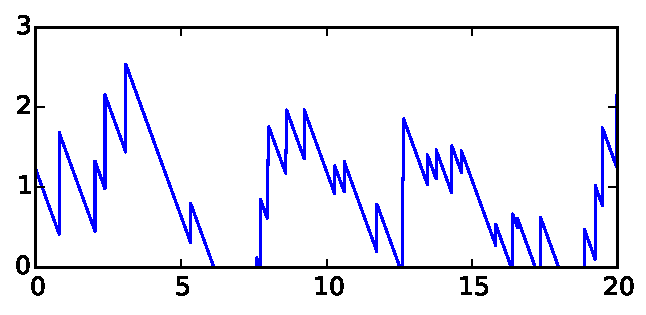
\includegraphics{virtualWaitingTime}
  \caption{The virtual waiting time $V(t)$ as  a function of time. }
  \label{fig:Virtual}
\end{figure}



Just as in Section~\ref{sec:constr-discr-time}, we again have
obtained a set of recursions by which we can run a simulation of a
queueing process of whatever length we need, provided we have a
sequence of have inter-arrival times $\{X_k\}$ and service times
$\{S_k\}$.  A bit of experimentation with computer programs such as
$R$ or python reveals that this is easy.


As an example on the type of conclusions we can draw from using the
above recursions, take $\{X_k\}$ and $\{S_k\}$ as in
Exercise~\ref{ex:5}. Starting with $W_{Q,0}=5$ we use
Eq.~(\ref{eq:56}) to compute the distribution of $W_{Q,k}$ for
$k=1,2,\ldots 20$, c.f., the left panel in
Figure~\ref{fig:convergence} for the results. Here we see that when
$k=5$, the `hump' of $\P{W_{Q,5}=x}$ around $x=5$ is due the starting
value of $W_{Q,0}=5$. However, for $k>10$ the distribution of
$W_{Q,k}$ hardly changes, at least not visually. Apparently, the
convergence of the sequence of distributions of $W_{Q,k}$ is rather
fast. In the middle panel we show the results of a set of simulations
for increasing simulation length, up to $N=1000$ samples. Here we also
see that the distribution to be defined in Eq.~(\ref{eq:48}) converges
quite fast to some limiting function. Finally, in the right hand panel
we compare the densities as obtained by the exact method and
simulation. Clearly, for all practical purposes, these densities can
be treated as the same.

The most important lesson of these experiments is that the convergence
of the random variables $W_{Q,k}$ to some the steady-state random
variable $W$ appears to be rather fast. This validates, to some
extent, that most queueing theory is concerned with the analysis of
the system in \emph{stationarity}. As a matter of fact, the study of
queueing systems in stationary state will occupy us for the rest of
these notes.


\begin{figure}
  \centering
  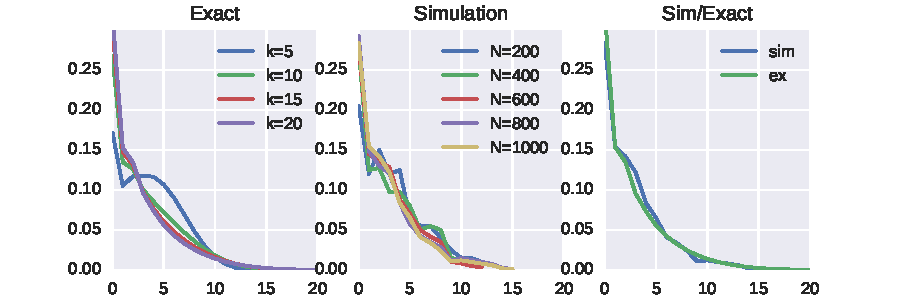
\includegraphics{gg1convergence}
  \caption{The density of $W_{Q,k}$ for $k=5, 10, 15, 20$ computed by
    an exact method as compared the density obtained by simulation of
    different run lengths $N=200, 400, \ldots 1000$. The right panel
    compares the exact density of $W_{Q,20}$ to the density obtained by simulation
    for $N=1000$.}
\label{fig:convergence}
\end{figure}



\begin{question}
  \begin{enumerate}
  \item Assume that $X_1=10$, $X_2=5$, $X_3=6$ and $S_1 = 17$,
    $S_2=20$ and $S_3=5$, compute the arrival times, waiting times in
    queue, the sojourn times and the departure times for these three
    customers.
  \end{enumerate}
  \begin{solution}
     The intent of this exercise is
      to make you familiar with the notation.

      BTW, such simple test cases are also very useful to test
      computer code. The numbers in the exercise are one such simple
      case. You can check the results by hand; if the results of the
      simulator are different, there is a problem.
    \end{solution}
  \end{question}
  
\begin{question}
 What are  the meanings of $A_{A(t)}$ and $A(A_n)$?
 \begin{solution}
  $A(t)$ is the number of arrivals during $[0,t]$. Suppose that
    $A(t) = n$. This $n$th job arrived at time $A_n$. Thus, $A_{A(t)}$
    is the arrival time of the last job that arrived before or at time
    $t$. In a similar vein, $A_n$ is the arrival time of the $n$th
    job. Thus, the number of arrivals up to time $n$, i.e., $A(A_n)$,
    must be $n$.
  \end{solution}
\end{question}


\begin{question}
  Define $L_Q(t)$ as the number of job in queue, and $L_s(t)$ as the
  number of jobs in service. Likewise, let $D_Q(t)$ be the number of
  jobs that departed from the queue up to time $t$.
  \begin{enumerate}
  \item Why don't we need separate notation for $D_s(t)$, the number
    of jobs that departed from the server? 
  \item Is $D_Q(t) \leq D(t)$ or $D_Q(t) \geq D(t)$?
  \item Why is $L(t) = L_Q(t) + L_s(t)$?
  \item Express $L_Q(t)$ and $L_s(t)$ in terms of $A(t)$, $D_Q(t)$ and $D(t)$.
  \item Consider a multi-server queue with $m$ servers. Suppose that
    at some $t$ it happens that $D_Q(t) - D_s(t) < m$ even though
    $A(t) - D_s(t) > m$. How can this occur? 
  \end{enumerate}
\begin{solution}
  \begin{enumerate}
  \item Because $D_s(t) = D(t)$. Once customers leave the server,
    their service is completed, and they leave the queueing system.
  \item All customers that left the system must have left the
    queue. Thus, $D_Q(t) \geq D(t)$.
  \item Jobs in the system are in queue or in service.
  \item $L_Q(t) = A(t) - D_Q(t)$. $L_S(t) = D_Q(t) - D(t)$. This is in
    line with the fact that $L(t) = L_Q(t) + L_s(t) = A(t) - D(t)$.
  \item In that case, there are servers idling while there are still
    customers in queue. If such events occur, we say that the server
    is not work-conservative.
  \end{enumerate}
\end{solution}
\end{question}



\begin{question}
  \begin{enumerate}
  \item 
  Show that $L(t) = A(t)-D(t)$ implies that 
  \begin{equation*}
    L(t) = \sum_{k=1}^\infty \1{A_k \leq t < D_k}.
  \end{equation*}
\item Show that if $L(A_k)>0$, i.e., the system contains at least one
  job at the time of the $k$th arrival, then $A_k \leq D_{k-1}$, i.e.,
  job $k$ arrives before job $k-1$ departs.
  \end{enumerate}
\begin{solution}
  \begin{enumerate}
  \item 
  \begin{equation*}
    \begin{split}
      L(t)
&= A(t) - D(t) \\
&= \sum_{k=1}^\infty \1{A_k \leq t} -  \sum_{k=1}^\infty \1{D_k \leq t} \\
&= \sum_{k=1}^\infty [\1{A_k \leq t} -  \1{D_k \leq t}].
    \end{split}
  \end{equation*}
  Write for the moment $A=\1{A_k \leq t}$ and
  $\bar A = 1- A = \1{A_k > t}$, and likewise for $D$. Now we can use
  Boolean algebra to see that
  $\1{A_k \leq t} - \1{D_k \leq t} = A-D = A(D+\bar D) -D = AD +
  A\bar D - D = A\bar D - D(1-A) = A\bar D - D \bar A$.
  But $D \bar A = 0$ since
  $D \bar A = \1{D_k \leq t} \1{A_k > t} = \1{D_k \leq t < A_k}$
  which would mean that the arrival time $A_k$ of the $k$th job would
  be larger than its departure time $D_k$. As $A \bar D = \1{A_k \leq t < D_k}$
  \begin{equation*}
    \begin{split}
      L(t)
&= \sum_{k=1}^\infty [\1{A_k \leq t} -  \1{D_k \leq t}] \\
&= \sum_{k=1}^\infty \1{A_k \leq t < D_k}.
    \end{split}
  \end{equation*}

  Boolean algebra is actually a really nice way to solve logical
  puzzles. If you are interested you can find some examples on my
  homepage. 
\item In a sense, the claim is evident, for, if the system contains a
  job when job $k$ arrives, it cannot be empty. But if it is not
  empty, then at least the last job that arrived before job $k$, i.e.,
  job $k-1$, must still be in the system. That is, $D_{k-1} \geq A_k$. A more formal proof proceeds along the following lines. Using that $A(A_k) = k$ and $D(D_{k-1})= k-1$, 
  \begin{equation*}
    \begin{split}
      L(A_k) &> 0 \Leftrightarrow A(A_k) - D(A_k) > 0   \Leftrightarrow k - D(A_k) > 0 \Leftrightarrow k > D(A_k) \\
      &\Leftrightarrow k-1 \geq D(A_k) \Leftrightarrow D(D_{k-1}) \geq D(A_k) \Leftrightarrow D_{k-1} \geq A_k, 
    \end{split}
  \end{equation*}
  where the last relation follows from the fact that $D(t)$ is a
  counting process, hence monotone non-decreasing.
  \end{enumerate}

\end{solution}
\end{question}



\begin{question}
  \begin{enumerate}
  \item 
  The definition of $L_k$ in Eq.~(\ref{eq:55}) is, algorithmically
  speaking, quite inefficient: for each $k$ we count all departures
  from $i=1$ all the way up to $k-1$. The following is more efficient: 
  \begin{equation*}
    L_k = L_{k-1}+1 - \sum_{i= k-1 - L_{k-1}}^{k-1} 1\{D_i< A_k\}.
  \end{equation*}
  Can you derive this?
\item Why do we take $i=k-1-L_{k-1}$ in  the sum, and not $i=k-2-L_{k-1}$?
\end{enumerate}
\begin{solution}
  \begin{enumerate}
  \item 
  Let $L_{k} = L(A_{k}-)$, i.e., the number of jobs in the system as
  `seen by' job $k$. It must be that $L_{k}=k-1 - D(A_{k})$. To see
  this, assume first that no job has departed when job $k$
  arrives. Then job $k$ must see $k-1$ jobs in the system. In general,
  if at time $A_k$ the number of departures is $D(A_k)$, then the
  above relation for $L_k$ must hold. Applying this to job $k-1$ we get that $L_{k-1} = k-2 - D(A_{k-1})$. 

  For the computation of $L_k$ we do not have to take the departures
  before $A_{k-1}$ into account as these have already been
  `incorporated in' $L_{k-1}$.  Therefore,
  \begin{equation*}
    L_k = L_{k-1} + 1 - \sum_{i= k-1 - L_{k-1}}^{k-1} 1\{D_i< A_k\}.
  \end{equation*}
\item 
    Suppose $L_{k-1}=0$, i.e., job $k-1$ finds an empty system at its
    arrival and $D_{k-1}>A_{k}$, i.e., job $k-1$ is still in the
    system when job $k$ arrives. In this case, $L_{k}=1$, which checks
    with the formula.  Also, if $L_{k-1}=0$ and $D_{k-1}< A_k$ then
    $L_k = 0$. This also checks with the formula. 

    The reason to start at $k-1-L_{k-1}$ is that the number in the
    system as seen by job $k$ is $k-1 - D(A_k)$ (not
    $k-2-D(A_k)$). Hence, the jobs with index from
    $k-1-L_{k-1}, k-L_{k-1}, \ldots, k-1$, could have left the system
    between the arrival of job $k-1$ and job $k$.

\TBD: check with simulation.
\end{enumerate}
\end{solution}
\end{question}


\begin{question}
  Provide a specification of the virtual waiting time process $\{V(t)\}$ for
    all $t$.
    \begin{solution}
      There is a funny way to do this. Recall from a previous exercise
      that if $A(t)=n$, then $A_n$ is the arrival time of the $n$th
      job. Thus, the function $A_{A(t)}$ provides us with arrival
      times as a function of $t$. When $t=A_{A(t)}$, i.e., when $t$ is
      the arrival time of the $A(t)$th job, we set
      $V(t) = V(A_{A(t)}) = W_{A(t)}$ i.e., the virtual waiting time
      at the arrival time $t=A_{A(t)}$ is equal to the waiting time of
      the $A(t)$th job. Between arrival moments, the virtual waiting
      time decreases with slope $1$, until it hits 0.  Thus,
      \begin{equation*}
        V(t) 
= \max\{V(A_{A(t)}) + (A_{A(t)}-t), 0\} 
= \max\{W_{A(t)} + (A_{A(t)}-t), 0\}.
      \end{equation*}
      The notation may be a bit confusing, but it is in fact very
      simple. Take some $t$, look back at the last arrival time before
      time $t$, which is written as $A_{A(t)}$. (In computer code these
      times are easy to find.) Then draw a line with slope $-1$ from
      the waiting time that the last arrival saw.
    \end{solution}
\end{question}




\begin{question}

  Another set of recursions to compute the arrival and departure times
  for a given set of inter-arrival and service times is the following:
\begin{equation}
  \label{eq:45}
  \begin{split}
    A_k &= A_{k-1} + X_k, \\
    D_k &= \max\{A_k, D_{k-1}\} + S_k.
  \end{split}
\end{equation}
Now the computation of the waiting times is trivial:
$W_k = D_k - A_k$.
  \begin{enumerate}
  \item Why do the recursions Eq.~(\ref{eq:45}) work? 
  \item  (Difficult) Extend the above recursions to a situation in which one queue is
  served by two servers.  
\item (Very hard) Extend the above recursions to a situation in which
  one queue is served by $m>2$ servers.
\item (Impossible?) As a real challenge you can attempt to extend these recursions to
  a situation in which the two servers have different working
  rates. (I don't know whether this can be done, though, without using
  a full-fledged simulator.)
  \end{enumerate}
  \begin{solution}
    \begin{enumerate}
    \item Of course, the service of job $k$ cannot start before it
      arrives. Hence, it cannot leave before $A_k + S_k$. Therefore it
      must be that $D_k \geq A_k +S_k$. But the service of job $k$ can
      also not start before the previous job, i.e. job $k-1$, left the
      server. Thus job $k$ cannot start before $D_{k-1}$. To clarify
      it somewhat further, define $S_k'$ as the earliest start of job
      $k$. Then it must be that $S_k' = \max\{A_k, D_{k-1}\}$---don't
      confuse the earliest start $S_k'$ and the service time
      $S_k$---and $D_k = S_k' + S_k$.
    \item I found this not easy, to say the least\ldots The problem is
      that in a multi-server queueing systems, unlike for
      single-server queues, jobs can overtake each other: a small job
      that arrives after a very large job can still leave the system
      sooner. After trying for several hours, I obtained an inelegant
      method. A subsequent search on the web helped a lot. The
      solution below is a modification of N. Krivulin, `Recursive
      equations based models of queueing systems'. 

The recursions for the two-server system are this: 
      \begin{equation*}
        \begin{split}
          A_k &= A_{k-1} + X_k, \\
          C_k &= \max\{A_k, D_{k-2}\} + S_k,\\
          M_k &= \max\{M_{k-1}, C_k\}, \\
          D_{k-1} &= \min\{M_{k-1}, C_k\}.
        \end{split}
      \end{equation*}
      Here, $C_k$ is the completion time of job $k$, and $\{D_k\}$ is
      a sorted list of departure times. Thus, $D_k$ is the $k$th
      departure time; recall this is not necessarily equal to the
      completion time $C_k$ of the $k$th job (as jobs may overtake
      each other). To understand the other equations, we reason like
      this.  By construction, $C_k > D_{k-m}$ (as $S_k >0$).
      Therefore, when we arrived at time $C_k$, $(k-m)$ jobs must have
      departed. Moreover, by construction, $M_k$ tracks the latest
      completion time of all $k$ jobs, hence, $M_{k-m+1}$ is the latest
      completion time of the first $k-m+1$ jobs. Therefore, if
      $C_k>M_{k-1}$, job $k$ must leave later than the latest of the
      jobs in $\{1,2,\ldots, k-1\}$.  Hence, the latest departure time
      of the jobs in $\{1, 2, \ldots, k-1\}$ jobs must be
      $M_{k-1}$. If however, $C_k<M_{k-1}$, then job $k$ leaves
      earlier than the latest of the jobs in $\{1,2,\ldots, k-1\}$. As
      $C_k>D_{k-2}$, it must be that $C_k > M_{k-2}$, because
      $D_{k-2}$ is latest departure of the jobs in
      $\{1,2,\ldots, k-2\}$, and this is also equal to $M_{k-2}$. As a
      consequence, if $C_k < M_{k-1}$, job $k$ is also the first job
      that leaves after $D_{k-2}$ ( provided of course that
      $C_{k+1} < C_k$). Thus, all in all
      $D_{k-1} = \min\{M_{k-1}, C_k\}$.
\item Similar reasoning for the $G/G/m$ queue leads to the following.
      \begin{equation*}
        \begin{split}
          A_k &= A_{k-1} + X_k, \\
          C_k &= \max\{A_k, D_{k-m}\} + S_k,\\
          M_k &= \max\{M_{k-m+1}, C_k\}, \\
          D_{k-m+1} &= \min\{M_{k-m+1}, C_k\}.
        \end{split}
      \end{equation*}
    This is not correct, though. Can you find a counter example?
  \item See my remark in the exercise. I think it is somewhere between
    too hard and impossible.
    \end{enumerate}
  \end{solution}
\end{question}




\begin{question}
  Implement the above recursions in excel or some other computer
  program such as R or python and check the results of the previous
  exercise.
    \begin{solution}
      Below I include three versions, one in python, one in R and one
      in Julia. Take your pick, and start playing with it. These
      examples are meant to be simple to understand, not necessarily
      super efficient.  

In python:

<<evaluate =  False>>=
import numpy as np
from numpy.random import exponential
import matplotlib.pylab as plt

N = 10
labda, mu = 2, 3

A = np.zeros(N)
D = np.zeros_like(A)
W = np.zeros_like(A)

for k in range(1, N):
    Xk = exponential(1. / labda)
    Sk = exponential(1. / mu)
    A[k] = A[k - 1] + Xk
    D[k] = max(A[k], D[k - 1]) + Sk
    W[k] = D[k] - A[k]
@
  
In R: 

<<evaluate=False>>=
N <- 10
lambda <- 2
mu <- 3

A <- rep(0, N)
D <- rep(0, N)
W <- rep(0, N)

for(k in 2:N){
  Xk <- rexp(1,lambda)
  Sk <- rexp(1,mu)
  A[k] <- A[k-1] + Xk
  D[k] <- max(A[k], D[k-1]) + Sk
  W[k] <- D[k] - A[k]
}
print(W)
@

In Julia:
<<evaluate=False>>=
N = 10
lambda, mu = 2, 3

arrival = zeros(N) #absolute time of arrival
departure = zeros(N) #absolute time of departure
waiting_time = zeros(N)

for k in 2:N
    time_to_arrival_k = rand(Exponential(1. / lambda)) #time between arrival k-1 and k
    service_time_k = rand(Exponential(1. / mu))
    arrival[k] = arrival[k - 1] + time_to_arrival_k
    departure[k] = max(arrival[k], departure[k - 1]) + service_time_k
    waiting_time[k] = departure[k] - arrival[k]
end
print(waiting_time)
@

\end{solution}
\end{question}

\begin{question}
  Validate the results of  Figure~\ref{fig:convergence} with simulation.
  \begin{solution}
    This is the code I used. You can study it if you like, but
    skipping it is OK, as is always the case with the code I include.


<<evaluate=False>>=
from collections import Counter
from matplotlib.pylab import plt
import seaborn as sns
sns.set_context("paper")

from lea import Lea

W0 = 5  # Lea.fromVals(0, 1, 2)
S = Lea.fromVals(1,  2, 3)
X = Lea.fromVals(1,  2, 4)
U = S - X

def simulate():
    count = Counter()
    N = 1000
    W = max(W0 + U.random(), 0)
    for k in range(1, N + 1):
        W = max(W + U.random(), 0)
        count[W] += 1
        if k % (N // 5) == 0: # make 5 plots
            x = [w for w in count]
            tot = sum(count.values())
            y = [count[w] / tot for w in count]
            plt.plot(x, y, label="N={}".format(k))
    return x, y


def exact():
    W = Lea.fastMax(W0 + U, 0)
    for k in range(1, 21):
        if k % 5 == 0:
            plt.plot(W.support(), W.pmf(), label="k={}".format(k))
        W = Lea.fastMax(W + U, 0)
    return W.support(), W.pmf()


plt.figure(figsize=(6, 2))

plt.subplot(131)
plt.axis([0, 20, 0, 0.3])
plt.title("Exact")
xex, yex = exact()
plt.legend()


plt.subplot(132)
plt.axis([0, 20, 0, 0.3])
plt.title("Simulation")
xsim, ysim = simulate()
plt.legend()

plt.subplot(133)
plt.axis([0, 20, 0, 0.3])
plt.title("Sim/Exact")
plt.plot(xsim, ysim, label="sim")
plt.plot(xex, yex, label="ex")
plt.legend()

# plt.show()
filename = "figures/gg1convergence.pdf"
plt.savefig(filename)
@

\end{solution}
\end{question}

\begin{question}(Multiple queues) Suppose one server serves two
  queues, such that jobs in queue A are served with priority over jobs
  in queue B. Assume that service is not-preemptive.  Can you develop
  a similar set of recursions for each of the queues, or, otherwise,
  an algorithm?
  \begin{solution}
    This question came up in class. I don't think this can be
    constructed as a straightforward recursion, and a search on the
    web lead to nothing. In case you can find a recursion, please let
    me know.  

    While a straightforward recursion may not exist, it is not really
    difficult to code this queueing discipline. The key idea is to put
    all jobs into one queue, but sort the elements in the queue in
    order of priority. Every time the server becomes empty, it checks
    the head of the queue. If the queue is empty, it wait until the
    next arrival occurs. Otherwise, it starts the service of the first
    job in line. When a new job arrives, then identify its priority
    first, and then put it at the end of the jobs of the same
    priority.

    This type of sorting is known as lexicographic sorting, which is
    what we do when we build a dictionary. First we sort words in
    order of first letter, then the second letter, and so on. In case
    of sorting the queue, we first have to sort in order of priority,
    then, within the class of jobs with the same priority, sort in
    ascending order of arrival time.

    In python the code is like this, where I include the FIFO case for
    comparison. As always, it is not obligatory to memorize the  code.

<<evaluate=False>>=
class Fifo(Queue):
    def __init__(self):
        self.queue = SortedSet(key = lambda job: job.arrivalTime)

class Priority(Queue): # a priority queue
    def __init__(self, numServers = 1):
        self.queue = SortedSet(key = lambda job: job.p)
@

Interestingly, once we have a proper environment to carry out
simulations, changing the queueing discipline is a one-liner!.

  \end{solution}
\end{question}


\begin{question}(LIFO queue) Can you develop a set of recursions or
  algorithm for a LIFO (Last-In-First-Out) queue?
  \begin{solution}
    Again, I don't know a good set of recursions, but an algorithm is
    straightforward. Rather then sorting the jobs in queue in
    ascending order of arrival time, just sort them in descending
    order of arrival time. 


<<evaluate=False>>=
class Lifo(Queue):
    def __init__(self):
        self.queue = SortedSet(key = lambda job: -job.arrivalTime)
@

Another interesting queueing rule is to sort in increasing job size;
<<evaluate=False>>=
  class SPTF(Queue): # shortest processing time first
    def __init__(self):
        self.queue = SortedSet(key = lambda job: job.serviceTime)
@

Do you see how sort in descending order of job size (it just a matter
of putting a minus sign at the right place)?
  \end{solution}
\end{question}


%%% Local Variables:
%%% mode: latex
%%% TeX-master: "book"
%%% End:
